\documentclass[11pt,a4paper,oneside]{report}
\usepackage{moreverb}
\usepackage{graphicx}
\begin{document}
\title{SymPy, A Python Library for Symbolic Mathematics}
\author{Jason Hsu, Keyan Kousha, Damian Rooney}
\date{Fall 2011}
\maketitle
\section*{Introduction}
Manipulating mathematical equations in symbolic form is rarely a built-in general programming language (GPL) feature. It's certainly not in today's popular programming languages. For mathematicians, this means learning a new domain specific language (DSL) to conduct such work, often barring its functionality from use in a more general context. Where integration between a DSL and a GPL is possible, it is often complicated, or ugly at best; in addition, studying or modifying the code base in these frequently proprietary languages isn't allowed; and features normally found in a GPL are an afterthought and require learning additional new syntax. Beyond the inconvenience, most popular languages in the symbolic math domain also have prohibitive costs (e.g. MatLab, Mathematica, etc.). It would be nice then to have symbolic math be a library to a GPL, written in a GPL, licenced like a GPL, with an implementation as transparent as a GPL's implementation. This is where SymPy, an open source Python library for symbolic math, enters.
\section*{Features}
SymPy is both written and interfaced with entirely in Python (although, according to their webpage, in the future they will supply a C-written core as an option). It's feature list reads as you would expect a computer algebra system's (CAS) feature list to read. It provides things as basic as algebraic simplification and expansion, complex numbers, differentiation, integration, algebraic and differential equation solvers, etc. It also contains modules for algebraic geometry, arbitrary precision floating point arithmetic, statistics, matrices, and quantum physics, among others. Printing, and plotting in both two and three dimensions, is supported as well. SymPy furnishes the user with all the standard fare of a paid CAS, but for free in a well-known, non-proprietary language for easy extensibility and modification.\\\\
 SymPy's features have even found their way into a more elaborate open source CAS, Sage, which is similarly interfaced with via Python (however, unlike SymPy, Sage has components written in several other languages). According to Sage's Wikipedia entry, SymPy's library is used in it's implementation of calculus tools.
 \section*{The SymPy Core Package}
Naturally, the base classes for SymPy are fairly complex. But that affords an architecture that is straightforward yet powerful. Scratching a few surfaces is enough to get started using and extending SymPy.\\\\
The base class of all objects in SymPy, resident to the core package, is the Basic class. The Basic class encapsulates all functionality "basic" to all symbols. This includes defining things like comparisons between generic symbol trees, pattern queries, etc.; providing a uniform interface for accessing symbol object hashes, symbol atoms in expressions, and type info (like communitivity and positivity); and, insuring all symbols are immutable (more on that later). The Basic class is important because it's the parent to the Symbol class, which is the primary construct users interact with.
\subsection*{Symbol Objects}
To create a symbol in SymPy, one simply pulls up Python in interactive mode, imports the Symbol class from sympy and begins creating symbols as in the following:
\begin{verbatim}
>>> from sympy import Symbol
>>> a = Symbol('a')
>>> b = Symbol('b')
>>> c = a*b
>>> c
a*b
\end{verbatim}
What's shown above is pretty straightforward, but it demonstrates the simplicity of creating symbols then nesting them in an expression object of type Mul. Mul itself behaves much like a Symbol because it is similarly a descendant of Basic.
\begin{verbatim}
 |  Method resolution order:
 |      Mul
 |      sympy.core.operations.AssocOp
 |      sympy.core.expr.Expr
 |      sympy.core.basic.Basic
 |      sympy.core.assumptions.AssumeMeths
 |      sympy.core.evalf.EvalfMixin
 |      __builtin__.object
\end{verbatim}
This occurs because Symbol descends from a class that overloads the asterisk, and all other arithmetic operators, to deal with Symbols (synonymously in the architecture, Atoms and Exprs). Symbolic compositions like this extend to any class derived from Basic, so to enable users to define their own functions. A few more complicated uses/compositions are shown below, but many more exist and behave just as intuitively.
\begin{verbatim}
>>> from sympy import *
>>> from sympy.abc import x, a, b, c #creates Symbols for chars (more on this later)
>>> integrate(x**2 * exp(x) * cos(x), x)
x**2*exp(x)*sin(x)/2 + x**2*exp(x)*cos(x)/2 - x*exp(x)*sin(x) + exp(x)*sin(x)/2 
- exp(x)*cos(x)/2
>>> (pi*x**2 + x/3).evalf()
3.14159265358979*x**2 + 0.333333333333333*x
>>> x = Point(0,0)
>>> y = Point(c,0)
>>> z = Point(a,b)
>>> t = Triangle(x,y,z)
>>> t.area
b*c/2
>>> x = Symbol('x') #define x to be a symbol again
>>> limit(1/x, x, oo)
0
\end{verbatim}
The above should suffice for a top level understanding, but much else that exists in the core facilitates the movement, efficiency (there's a Symbol cache!), and representation of Symbols within SymPy.
\section*{Python in sympy.core}
Python is used in some interesting ways to acheive the core's functionality. We'll dicuss a small number of them briefly.
\subsection*{\_\_slots\_\_}
 One interesting way is keeping Basic and derived classes immutable and lightweight. This is done by interfering in the instance creation process.
\begin{verbatim}
    __slots__ = ['_mhash',              # hash value
                 '_args',               # arguments
                 '_assume_type_keys',   # assumptions typeinfo keys
                ]
\end{verbatim}
The above creates an immutable class by preventing the creation of the normal python dictionary, which would be extendable by users and take up unnecessary space. (All symbols in SymPy are also expression immutable, but this is kept by convention: always returning an "expression immutable" copy on mutate operations.)
\subsection*{\_\_new\_\_()}
Something else seen in this class Basic, and the majority of core classes, is the definition of \_\_new\_\_() which returns an instance of the class. Unlike \_\_init\_\_(), \_\_new\_\_() allows customization of the instance creation itself, not just initialization. One example of this is used to cache Symbol objects. The following is a return statement from Symbol's \_\_new\_\_().
\begin{verbatim}
return Symbol.__xnew_cached_(cls, name, commutative, **assumptions)
\end{verbatim}
This call returns a cached Symbol if it exists or creates a new Symbol should it not already exist, avoiding the recurrence of allocation. Singletons in SymPy are another, similar, instance of the use of \_\_new\_\_() which is used to check if a singleton is in the singleton registry.
\subsection*{Decorators}
Caches and registries aren't unique to Python; however, the way this is implemented in SymPy using Python is pretty attractive. In the case of caching, SymPy uses decorators to wrap function calls, the results of which are cached. In the Symbol class, this is done in the old style (closure syntax), but other occurences of the @cacheit decorator use this new style. 
\begin{verbatimtab}
# the occurence in sympy.core.symbol
__xnew_cached_ = staticmethod(cacheit(__new_stage2__))
# in sympy.core.basic
@cacheit
def _subs_old_new(self, old, new):
	...
\end{verbatimtab}
A common Python idiom is then used within @cacheit to ensure that this "wrapper" is transparent to the user of the function.
\begin{verbatimtab}
def __cacheit(func):
	...
	@wraps(func)
    def wrapper(*args, **kw_args):
    	...
    return wrapper
\end{verbatimtab}
This allows the interpreter to maintain the special attributes of \_subs\_old\_new, and other decorated functions, when the function being called is actually its wrapper (special attributes here are those such as \_\_name\_\_ and \_\_doc\_\_, which are important for introspection).
\subsection*{Metaclasses}
The last example that we'll cover on Python in SymPy's core, although are many, many more engaging uses, is metaclasses. Much like \_\_new\_\_ in Python intercepts instance creation of an object, metaclasses intercept creation of class objects. Everything in Python is an object, even ints, and so are classes.\\\\
 The class keyword internally creates an object for the specified there, and this is what metaclasses interfere with: how this class object is created. To interfere in this way, one simply defines the \_\_metaclass\_\_ variable in the class one wants to intevene in, and Python does the rest, calling the metaclass before the class object is created with the information about the original class object. The Basic class in sympy.core uses such a meta class. It's defined as simply as the following.
\begin{verbatim}
__metaclass__ = BasicMeta
\end{verbatim}
Being the base class for all symbol objects, Basic has many duties. One of these duties is maintaining assumptions about symbols and consequences derived from such assumptions. Metaclasses are inherited when subclassing, so as far as we can tell (admittedly, BasicMeta uses a lot of magic), BasicMeta creates default assumptions and derives consequences of premises that a class derived from Basic might define. This is the common use of metaclasses, often occuring in Python API's: abstraction of low-level class maintaince or representation for class designers.\\\\
As said, this is only a survey of a few Python tools used in SymPy's core package. But it should be clear how much of Python is being leveraged to do very cool things in its lower levels.
\section*{A SymPy Class Example}
SymPy leans heavily on Python features in its implementation. The result of this is clean, readable code. This in turn promotes one of the main goals of SymPy: extensibility.
\subsection*{Matrices}
The Matrix module of SymPy provides showcases several Python-specific features in action. For example, SymPy leverages Python's functional features to allow users to create matrices using "rules", which are essentially functions that populate the new matrix with values. The tidiness of this approach can be seen below:
\begin{verbatimtab}
        In [1]: Matrix(2, 2, lambda i,j: (i+2)*j )
        Out [1]: 
        ⎡0  2⎤
        ⎢    ⎥
        ⎣0  3⎦
\end{verbatimtab}
Accessing elements of a matrix also utilizes features of Python. In particular, SymPy matrices overload the braces operator to allow the user to intuitively address both individual elements or even entire submatrices. This is achieved by taking advantage of the slices operator built into Python:
\begin{verbatimtab}
        In [1]: A = Matrix(2, 2, lambda i,j: (i+2)*j )
        In [2]: A[0, :]
        Out [2]: [0, 2]
        In [3]: A[:, 1]
        Out [3]: 
        ⎡2⎤
        ⎢ ⎥
        ⎣3⎦
\end{verbatimtab}
Finally, SymPy implements several Python operators to create transparent matrix operations. To multiply two matrices, a user would simply apply the familiar * operator. However, SymPy internally achieves this by implementing Python's \_\_mul\_\_ and \_\_rmul\_\_ operators. This faithfully carries out matrix multiplication:
\begin{verbatimtab}
        In [4]: A = Matrix(1, 2, lambda i, j: (i+3)*j)
        In [5]: B = Matrix(1, 2, lambda i, j: (i+3))
        In [6]: A*B
        Out [6]: [0, 15]
\end{verbatimtab}
If the user tried to compute A*B, the operation would return an error due to the size mismatch between the matrices.
\section*{Formatting \& Printing in SymPy}
\subsection*{Features and Usage}
While SymPy’s symbolic math modules provide a fertile platform for a wide range of computational applications, the printing and formatting modules enable the results of those applications to be formatted correctly and shared easily. This is a very powerful feature facilitating mathematicians, scientists, and engineers to express their calculations in a human-readable form.\\\\
SymPy defines special terminology when it comes to printing and formatting. Foremost, printing an expression is not synonymous–in the traditional sense–with printing to paper or the screen; instead, it means that the expression is formatted and returned as a standard Python string. For the more conventional printing, SymPy offers a preview mode that outputs the expression as a rendered image, ready for a research report or presentation.\\\\
Printing relies on the polymorphic nature of Python to produce the correct output for any SymPy expression. To the end user, printing an expression involves just invoking the standard print function of Python. No special processing or compilation beforehand is required. The ease of use is illustrated below:
\begin{verbatimtab}
>>> from sympy import Integral
>>> from sympy.abc import x
>>> print x**2
x**2
>>> print 1/x
1/x
>>> print Integral(x**2, x)
Integral(x**2, x)
\end{verbatimtab}
Although unformatted plaintext is produced, a prettier representation can be achieved. In such cases, the pprint function of SymPy comes in handy. The following example demonstrates:
\begin{verbatimtab}
>>> from sympy import Integral, pprint
>>> from sympy.abc import x
>>> pprint(x**2)
 2
x
>>> pprint(1/x)
1
-
x
>>> pprint(Integral(x**2, x))
  /
  |
  |  2
  | x  dx
  |
 /
\end{verbatimtab}
SymPy also offers rich features for plotting data, putting it on par with commercial software such as MatLab and Mathematica. Plotting is achieved through Pyglet (a cross-platform windowing and multimedia library for Python) and called be controlled by console commands in addition to the keyboard and mouse.\\\\
SymPy supports several coordinate modes and color functions for each plotted function. A coordinate mode can be specified directly or automatically; Cartesian and parametric plots are automatically handled, leaving polar, cylindrical, and spherical modes requiring explicit specification. Custom color functions can also be added to enhance the look of the plot. The color functions can be specified by a multistep color gradient or separate functions for each component: red, green, and blue.\\\\
The following example demonstrates SymPy’s plotting functionality:
\begin{verbatimtab}
>>> from sympy import symbols, Plot, cos
>>> x,y = symbols('x y')
>>> Plot(cos(x*3)*cos(y*5)-y)
[0]: -y + cos(3*x)*cos(5*y), 'mode=cartesian'
\end{verbatimtab}
Figure 1: Output of plotting example
\begin{flushleft}
\begin{normalsize}
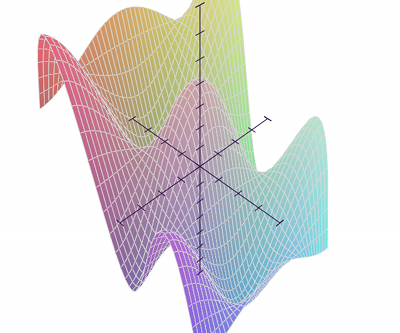
\includegraphics{plot.jpg}
\end{normalsize}
\end{flushleft}
\subsection*{Supported Outputs}
SymPy supports within its printing and formatting utilities a variety of output formats ranging from ASCII art to LaTeX and MathML. SymPy can also produce C and Fortran code as part of its printing and formatting capabilities. The C printer will try to use the standard C math libraries as much as possible. Of course, custom output formats can be implemented as well.\\\\
Figure 2: Examples of various output formats and their usage
\begin{verbatimtab}
>>> from sympy import Integral, latex
>>> from sympy.abc import x
>>> latex(x**2)
x^{2}
>>> latex(x**2, mode='inline')
$x^{2}$
>>> latex(x**2, mode='equation')
\begin{equation}x^{2}\end{equation}
>>> latex(x**2, mode='equation*')
\begin{equation*}x^{2}\end{equation*}
>>> latex(1/x)
\frac{1}{x}
>>> latex(Integral(x**2, x))
\int x^{2}\,dx
\end{verbatimtab}
(a) LaTeX output
\begin{verbatimtab}
>>> from sympy.printing.mathml import mathml
>>> from sympy import Integral, latex
>>> from sympy.abc import x
>>> print mathml(x**2)
<apply><power/><ci>x</ci><cn>2</cn></apply>
>>> print mathml(1/x)
<apply><power/><ci>x</ci><cn>-1</cn></apply>
\end{verbatimtab}
(b) MathML output
\begin{verbatimtab}
Fortran
>>> from sympy import *
>>> x = symbols("x")
>>> fcode(sqrt(1-x**2))
'      sqrt(-x**2 + 1)'
>>> fcode((3 + 4*I)/(1 - conjugate(x)))
'      (cmplx(3,4))/(-conjg(x) + 1)'
\end{verbatimtab}
(c) Fortran output
\section*{Applications of SymPy}
Outside of computer science, SymPy (and Computer Algebra Systems in general) has found a peculiar niche. Many practical applications of computational modeling rely on accurate numerical approximations of systems; SymPy doesn't excel at such tasks, as it has been designed for use in symbolic processing. However, SymPy's facilities are often a good fit for applications whose problems can be expressed in a closed, symbolic form.\\\\
One such field is quantum mechanics. Recently, there has been a fair amount of work put into the development of a SymPy module that has extended its algebraic aptitude to the realm of symbolic quantum mechanics. Through this module, SymPy users are now able to simulate quantum computation. This is achieved through the use of Qubit objects (which roughly correspond to quantum states), and Gate objects (which act on these states). Such simulations are useful to researchers in quantum computing; while actual quantum computers are as yet unachievable, researchers wishing to experiment with quantum algorithms would be well served by such simulations. (Cugini, June 2011)\\\\
SymPy has been used in another interesting application to quantum computing: programmatic simplification of quantum circuits. Without delving too deeply in the math, there is a quantum mechanical analogue to classical boolean logic gates. These operations on classical bits can sometimes be mirrored using "rotation-like operations in Hilbert space" on qubits (Curry, June 2011). This forms the theoretical basis for quantum computation.\\\\
Much like current logical circuits, it is important to find methods of creating efficient quantum circuits. This means minimizing the number of gates needed to implement a given logical expression. Work to create rules for systematically eliminating redundancies in quantum circuits has been undertaken, using SymPy's symbolic processing to derive such rules. (Curry, June 2011)
\end{document}